\documentclass[authoryear, 12pt,5p, times]{elsarticle}
%\usepackage[hypcap]{caption}
%\geometry{margin=0.95in,top=1.4in,bottom=1.4in}
\geometry{margin=1.1in,top=1.5in,bottom=1.5in}
\usepackage{float}
\usepackage{amsmath}
\usepackage[hidelinks]{hyperref} 
 \usepackage{gensymb}
\usepackage{subcaption}
\usepackage{url}
%\renewcommand\thefootnote{\fnsymbol{\dagger}}
\usepackage[symbol*]{footmisc}
\makeatletter
\newcommand{\rpm}{\raisebox{.3ex}{$\scriptstyle\pm$}}
\begin{document}
%\footnote{This is a footnote}
\begin{frontmatter}
\title{Doppler Measurement of Solar Rotation}
\author{\today \\ \quad \\Jung Lin (Doris) Lee\\  \href{mailto:dorislee@berkeley.edu}{dorislee@berkeley.edu} \\Group partners: Jennifer Ito, Manuel Silvia, Michael Hill\\Prof. James Graham, UGSI Heechan Yuk, Isaac Domagalski}
	\begin{abstract}
In this experiment, we captured the CCD images resulting from a spectrograph while the Sun drifts across the fiber aperture. We perform standard routine of dark, bias, and flat subtraction  and wavelength calibration using method of linear least squares. From the total intensity on the spectrometer during the full solar crossing, we determine the crossing time for each scan. We pre-process the 1D spectra by mean subtraction and weighing by window function and conduct cross correlation analysis on the datasets in the same scan with the mean spectra. Then, we convert this pixel shift to a observed velocity  at the solar limb using the pixel per wavelength factor acquired  from wavelength calibration and the Doppler velocity formula. We can deduce the velocity at the limb by multiplying the half crossing time by the gradient on a velocity-time graph plotted for the whole scan. Finally, we transform this observed velocity to the solar radial velocity to adjust for the non-zero viewing angle and the tilt of the solar spin axis. Repeating this analysis for 8 different solar scans yields the measurement of solar radial velocity as 1.257\rpm 0.0185 km/s  which translates to a solar radius of 453855 \rpm 6675 km.
	\end{abstract}
\end{frontmatter}
\section{Introduction}
Optical spectroscopy not only provides important information about the chemical composition observational targets but can also provide detailed insight into the orbital properties of planetary bodies from Doppler measurements on line features of a spectrum. Doppler spectroscopy of a parent star is a powerful method that can be used to deduce the properties of extrasolar planets that orbits around the star. Highly precise radial-velocity shifts can be achieved by  spectrographs such as the HARPS at La Silla Observatory in Chile to  look for smaller Earth-sized planets. The method of Doppler spectroscopy has revolutionized the field of exoplanet detection. 

In this lab, we explore the Doppler measurements of the rotation of our own star. This report present the methods and results obtained from the analysis of the Doppler shift between sets of spectra. In section \ref{hardwareexp}, I will present the spectroscope details and experimental setup for this experiment. In section \ref{data_reduction}, I will detail the various procedures that were used for data reduction as well as how we cross correlated sets of spectra to detect the Doppler shift signature. Finally, section \ref{results} presents how we arrive at the radial velocity and radius of the Sun from our cross correlation analysis and their associated errors. 
\section{Hardware and Experiment}
\label{hardwareexp}
\subsection{Experimental setup}
We point a 10cm, F/10, 4inch Newonian telescope at the Sun during noontime and 
an optical fiber is attached to the aperture of the telescope to lead the light to the spectrometer and data acquisition setup. After setting the telescope to point at a location close to the the Sun, we turn off the telescope's tracking motors and let the Earth's motion take over to take the drift scan. During the experiment, we made adjustments to the CCD exposure and the declination setup by looking at the data quality and length of the resulting scan. 
\subsection{Spectrometer details}
The spectrometer consists of a 300 mm$^{-1}$ transmission grating that disperses the collimated incident beam and a 80 mm${^-1}$ echelle grating  perpendicular to it. The resulting image captured by the APOGEE 13 $\mu$m CCD is a 1024 $\times$ 1024 image array with different orders of diffraction projected as a row spanning 20 nm across. 
\hspace{-20pt}
\begin{table}[h!]
    \begin{tabular}{|l|l|}
%    \hline
    \hline Angular dispersion [$m^{-1}$]  & 4.804                     \\      \hline Free spectral range [nm]           & 18.16                     \\     \hline Min wavelength [nm]  & 625.6
 \\  \hline  Max wavelength [nm]  &  643.76 
 \\ \hline Magnification   & 0.3357                
 \\ \hline       Angular dispersion [$m^{-1}$]  & 4.804                   \\ \hline   Spectral resolving power  & $1.317\times10^4$\\ 
    \hline Spectral resolution [km/s]   & 54.09        \\ 
   \hline Width on the CCD [mm]   & 0.52                      \\ \hline
    \end{tabular}
  
    \caption{Computed spectrometer information for $\lambda $=632.8 nm, corresponding to echelle order of  m=35. }
  \label{spec_prop}\end{table}

The spectral resolution in nm deals with the distance between two closely spaced features so that the features are resolved. This quantity can be computed by Eq. \ref{spectral_resolution} given in the lab handout.
\begin{equation}
\label{spectral_resolution}
\delta\lambda=\Bigg(\frac{\partial\lambda}{\partial\beta}\Bigg)_{m,\alpha}\Bigg(\frac{\partial\beta}{\partial\alpha}\Bigg)_{m,\lambda}\delta\alpha
\end{equation}
where $\Big(\frac{\partial\lambda}{\partial\beta}\Big)_{m,\alpha}$ is the reciprocal of the angular dispersion and $\Big(\frac{\partial\beta}{\partial\alpha}\Big)_{m,\lambda}$ is the anamorphic magnification computed as a ratio of the cosines of the incident and diffraction angles. The numerical result for the m=35 order is 3.629 pixels. Using the dispersion relation for pixel-to-wavelength conversion and the Doppler velocity formula described by Eq.\ref{doppler_eq}, we determine the resolution for the velocity measurement in km/s as cited in Table.\ref{spec_prop}.


\begin{figure}[h!]
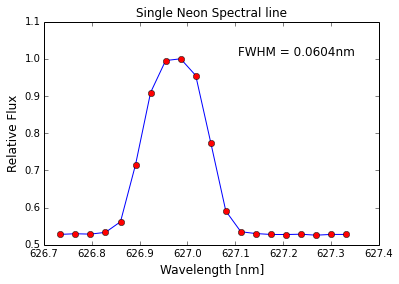
\includegraphics[width=0.5\textwidth]{figures/single_neon}
\caption{Above figure shows a single neon emission line. Since intensity distribution follows a normal distribution, the FWHM is computed by 2$\sigma\sqrt{2\ln(2)}$ where $\sigma$ is the standard deviation of cropped image containing a single neon line. Just like $\sigma$, the FWHM informs us about the width of a distribution. }
\label{fwhm}
\end{figure}
\subsection{Wavelength Calibration}
\begin{figure}[h!]
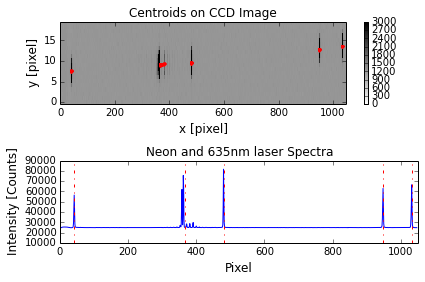
\includegraphics[width=0.5\textwidth]{figures/neon_spectra}
\caption{Top: Centroids of spectral lines of a single echelle order (m=35) on CCD. Bottom: CCD image converted to a 1D spectrum showing how the star-matching centroid algorithm in Lab \#3 yields accurate 1D pixel values for the spectral lines.}
\label{neon_spectra}
\end{figure}


\begin{figure}[h!]
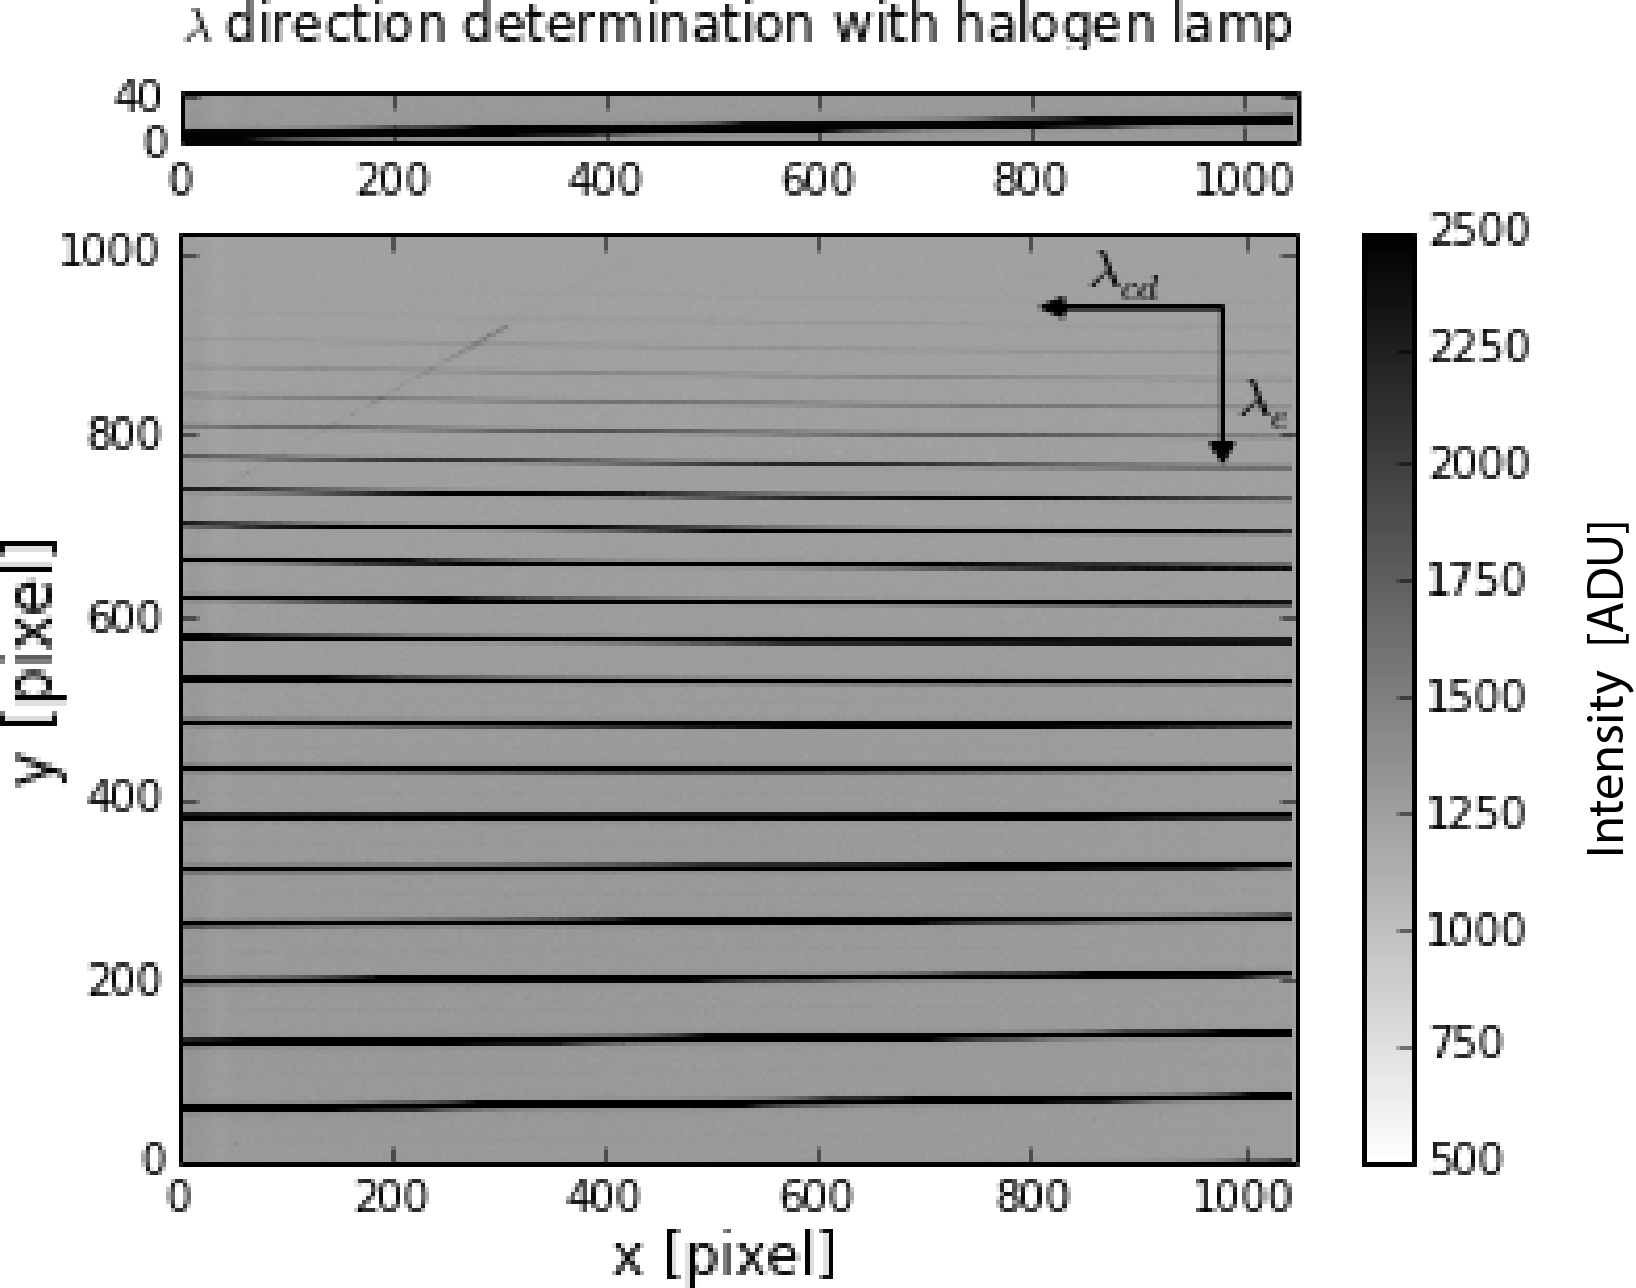
\includegraphics[width=0.5\textwidth]{figures/lambda_direction}
\caption{Wavelength direction, the arrow points in the direction of increasing wavelength. We determine the tilting direction from a zoomed-in section of a single echelle  order, as shown in the top figure.}
\label{lambda_direction}
\end{figure}
From the halogen spectrum we deduced that the cross-dispersion wavelength ( $\lambda_{cd}$) decreases along the direction of y axis and from the tilted order as shown in Fig.\ref{calib}, we conclude that the wavelength from the echelle grating ($\lambda_{e}$) increase from right to left.
We took exposures where both the neon light and 635nm green laser was turned on in order to identify the pixel location of the 35$^{\text{th}}$ order, as computed in Table \ref{spec_prop}.


By adopting the 1D and 2D centroid finding code in Lab \#2 and \#3, we find the centroid of the laser and neon lines on the CCD image as shown in Fig.\ref{neon_spectra}.  Using the method of linear least squares to match these pixel values with the Neon values obtained from NIST \footnote{The upper and lower wavelength should span the range of echelle order ($\approx 20nm$).} (with the manual addition of the given laser wavelength), we compute wavelength calibration on m=35 as: 
\begin{equation}
y = 0.03145 x + 625.6
\end{equation}
where x is in pixel units and y is in nm. Since each order has a slightly different coefficient, this equation is only applicable to orders of m=35 in every scan. 
 \begin{figure}[h!]
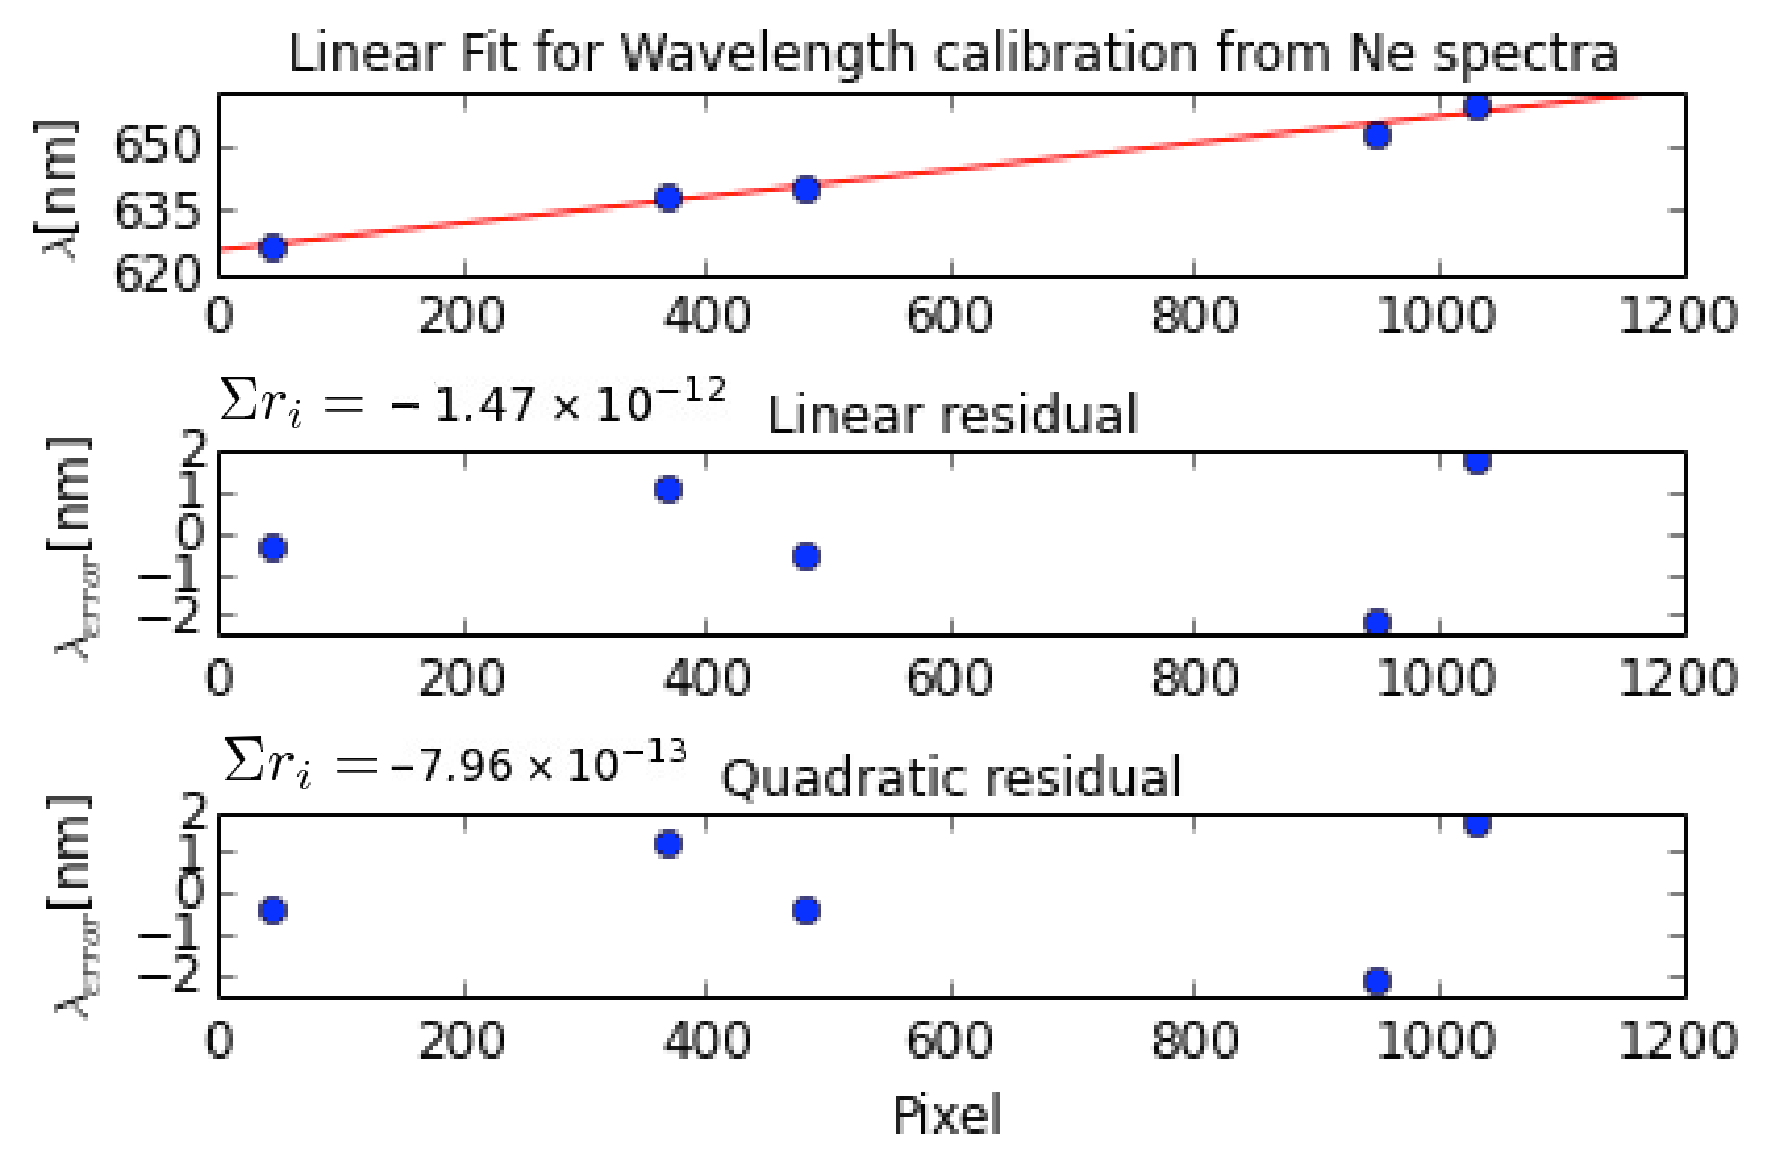
\includegraphics[width=0.5\textwidth]{figures/wavelength_calib}
\caption{The first order fit in the top figure shows that the dispersion is approximately linear ($\frac{d\lambda}{d\text{pixel}}$=0.0315 nm/pixel ). Since there is no notable patterns in linear residual and the magnitude of the residual is small, a linear relationship should be sufficient for pixel-to-wavelength conversion. From the bottom most quadratic figure, we see that the sum of the residual ($r_i$) decrease by an order of magnitude.}
\label{calib}
\end{figure}
\section{Data Reduction}
\label{data_reduction}
\subsection{Dark, Bias, Flat Subtraction}
\label{subtraction}
Using the halogen lamp as a source of uniform illumination, the flat field images calibrate the pixel-by-pixel variations as well as common artifacts seen in both continuum sources as shown in Fig.\ref{processed}. We take the ``dark frame" as the the average of the frames (i.e. the flat region shown in Fig.\ref{eddington_fit}) before and after the solar crossing. Without subtracting the bias in the ``dark image", we can automatically get bias subtraction by simply subtraction off the dark, as the bias is incorporated as part of the ``dark frame" .
Every image pixel is processed by:
\begin{equation}
			\frac{\text{image}-\text{dark}}{\text{flat}}\times\text{median(flat)}
			\label{calib_eq}
\end{equation}
 When converting the 2D images to 1D spectra, we took a 1024-by-1024 pixel slice of the image array to truncate the 24 overscan pixels.
 \begin{figure}[h!]
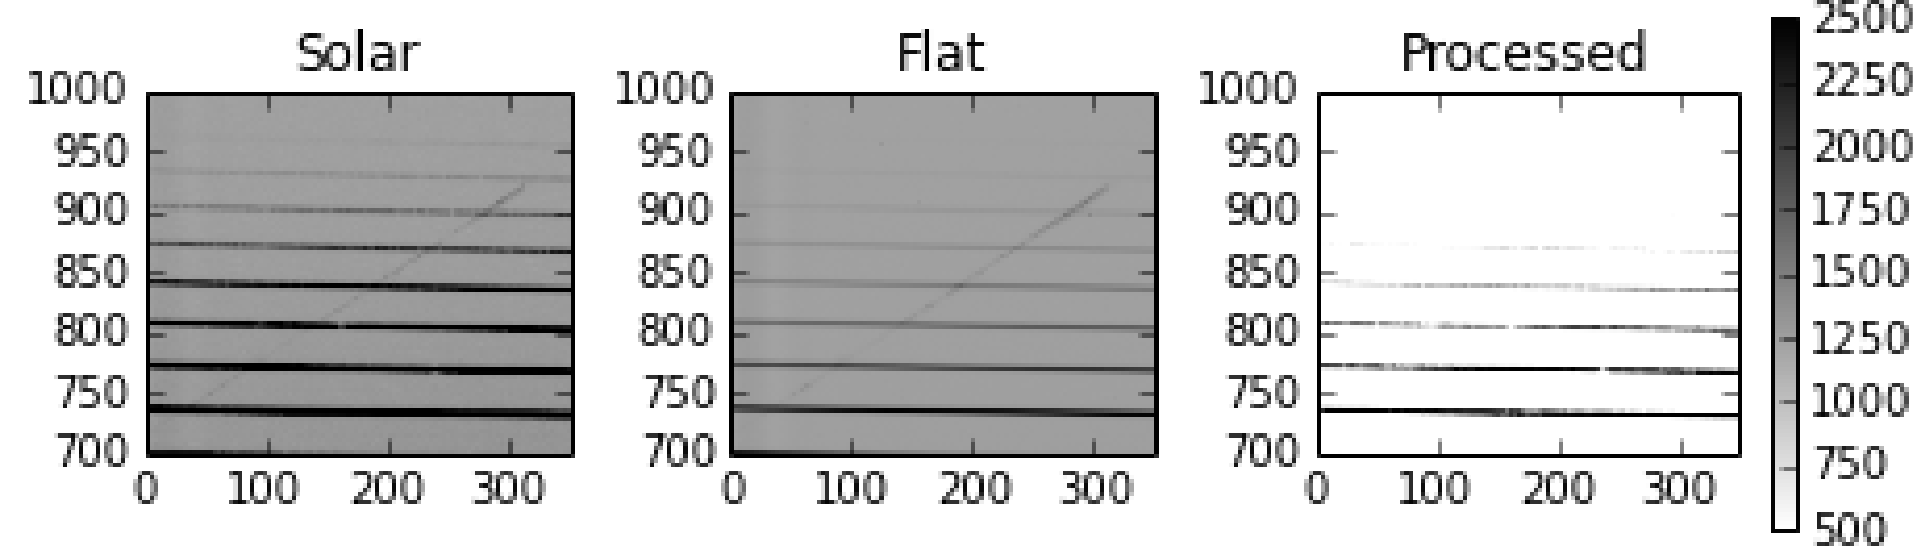
\includegraphics[width=0.5\textwidth]{figures/processed}
\caption{Both continuous sources shows the same artifact in a corner of the CCD image. The figures below are zoomed in on this feature, which  possibly originates from the stray, reflected light in the black box containing the spectrometer and CCD. The halogen exposure is used for flat correction. Along with subtracting the background from the non-incident solar spectrum, the artifact is removed in the processed image shown in the rightmost figure.}
\label{processed}
\end{figure}
\subsection{Limb Darkening}
The data quality of the solar scan can be verified by the a time series plot as shown in Fig.\ref{eddington_fit}. Intensity fluctuation that deviates from the predicted effect of limb darkening indicates possible shading effect from presence of cloud or objects near the telescope such as a crossing observer. Qualitatively, this information can be used to visually reject entire shaded scans or pick out exposures in the bright central region for a more accurate Doppler shift determination. Quantitatively, we can also make use of the limb darkening effect to determine crossing time of the solar scan, used in our solar angular size calculation in Sec.\ref{size_calc}.

We see the effect of limb darkening by summing together the intensity of all pixel in every CCD image in a full solar scan. Limb darkening results from the fact that an observer can only see through a constant optical depth of 2/3. As the density and temperature of a star decreases radially outwards, the observer sees light originating from different regions of the star,thus the cooler, less dense regions at the limb corresponds to the darkening effect. 

The time series data in Fig.\ref{eddington_fit} shows the total intensity of each exposure scaled by the intensity at the central bright peak ($I_0$) which we set as the origin. By modelling intensity as a function of the incident viewing angle using the Eddington approximation for grey, plane-parallel stellar atmosphere, we obtain the relation\footnote{See derivation from lab handout. Also, see Ch 9.4 in Caroll and Ostlie (2007)} 
\begin{equation}
\frac{I(\theta)}{I(\theta=0)}=\frac{I}{I_0}= \frac{2}{5}+\frac{3}{5}cos\theta
\label{eddington_eq}
\end{equation}
By geometrically relating this with the Earth-sun distance and crossing times, we get: 
\begin{equation}
\cos \theta = \sqrt{1-(t-t_0)^2/\Delta t^2} 
\end{equation}
where $t_0$ is where the time of the central bright peak, t is the time of each scan and $\Delta t$ is the crossing time.


\begin{figure}[h!]
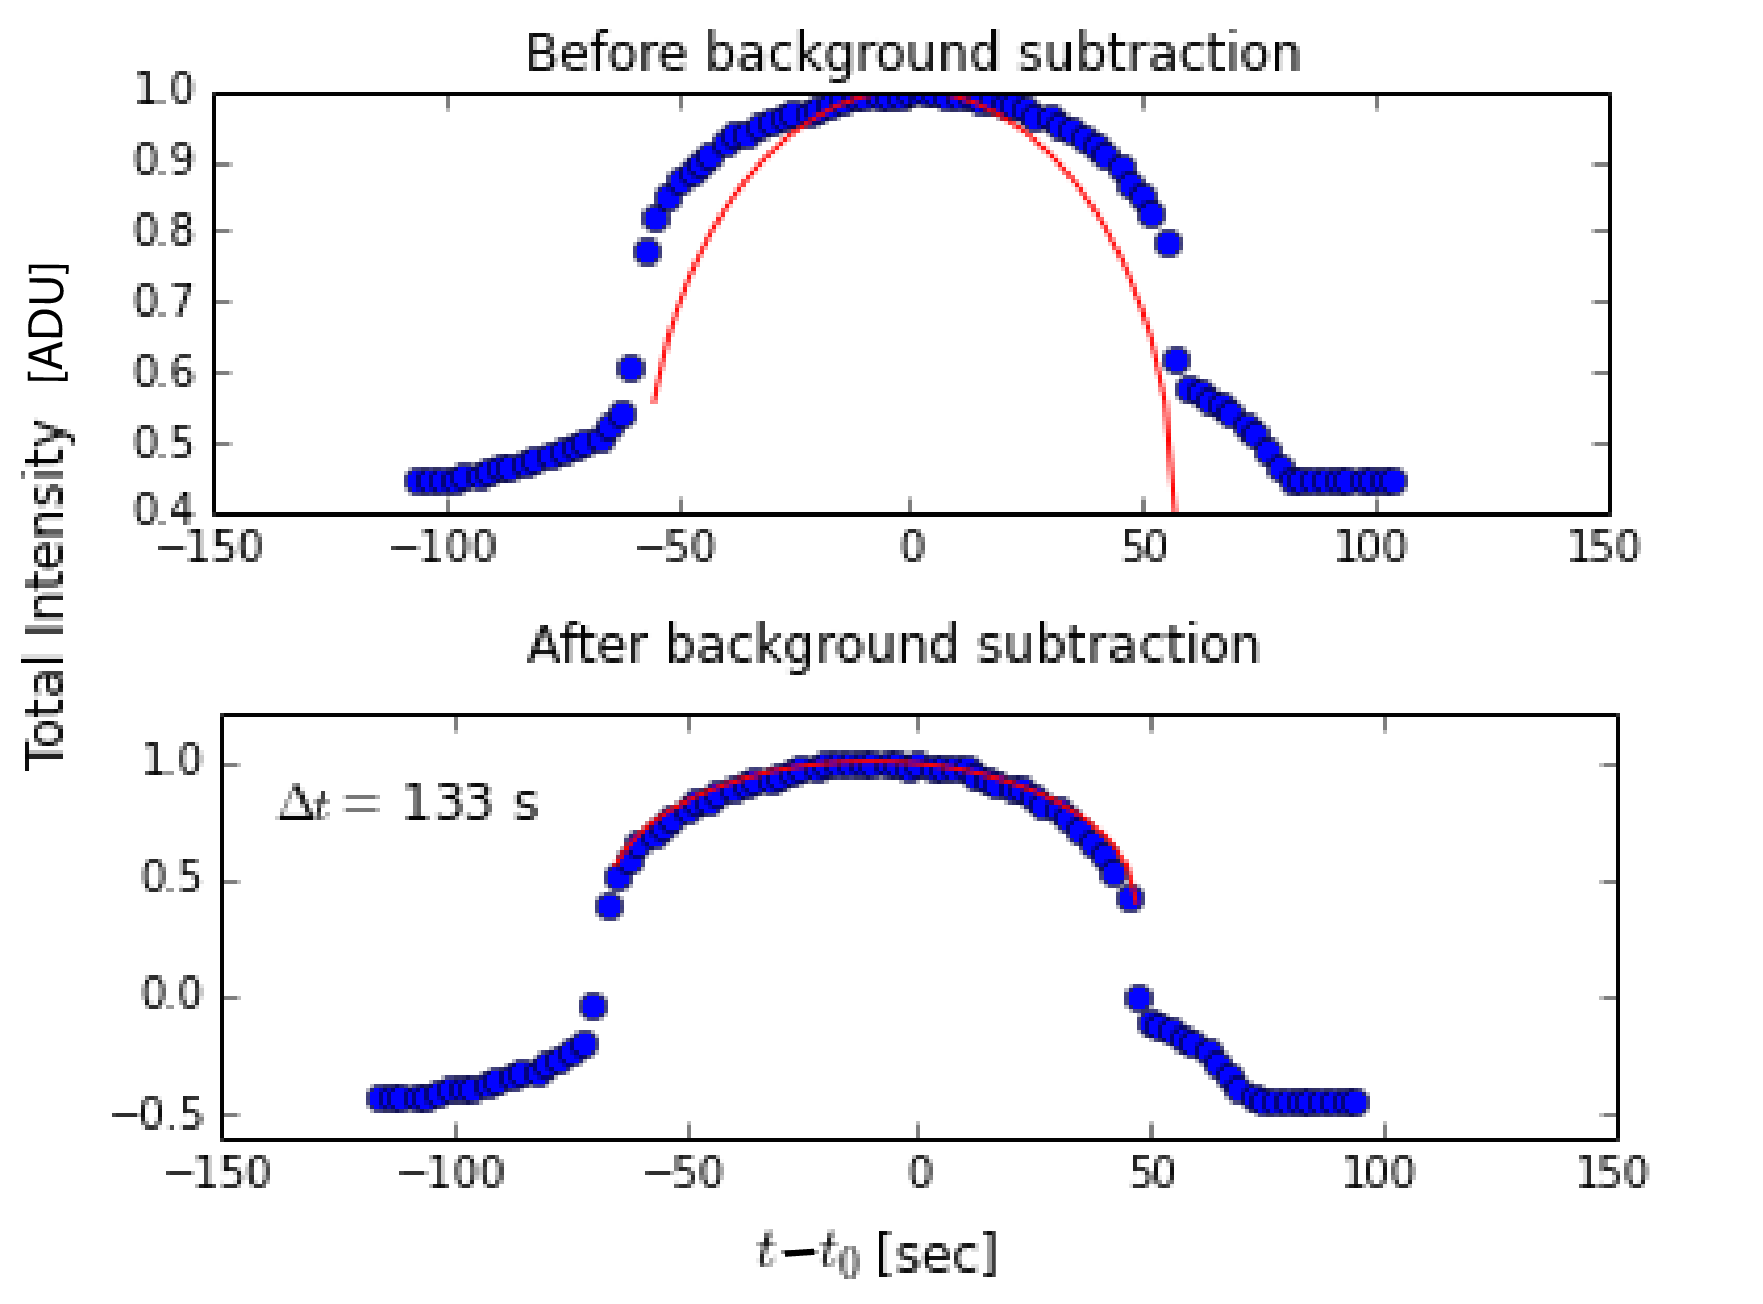
\includegraphics[width=0.5\textwidth]{figures/eddington_fit}
\caption{ The y-axis is normalized so that curve fitting corresponds to the model's output I/$I_0$ . The clear improvement of the model fit after background subtraction is evident as some of the intensity fluctuation may be mitigated by systematic effects corrected in the dark and flat frames discussed in Sec.\ref{subtraction}.}
\label{eddington_fit}
\end{figure}

To avoid the arbitrary determination of the exposure that defines the start and end of the solar crossing, we fit our data to Eq.\ref{eddington_eq} with the crossing time ($\Delta t$) as our varying parameter.  The lower figure in Fig.\ref{eddington_fit} shows the result of substituting the value of $\Delta t$ back into Eq.\ref{eddington_eq}, and ignoring the uneven data points on the two sides  (an artifact of the telescope) as well as regions before and after the solar crossing. Without this procedure, the fit would be largely distorted by the telescope artifact on the two sides and the ``dark" regions, which is not part of the stellar model.  Note that the lower fit in Fig.\ref{eddington_fit} also does not fully include the first two scans after the jump, yielding a more accurate estimate for the crossing time. This way of defining the boundaries of the stellar atmosphere is a more robust method than simply selecting the datapoint where the jump in intensity occurs and computing $\Delta t$ from the FITS header time information.


\subsection{Cross-Correlation Analysis}
\begin{figure}[h!]
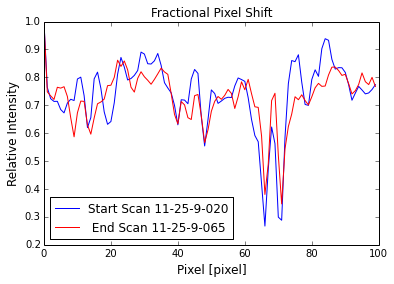
\includegraphics[width=0.5\textwidth]{figures/pix_shift}
\caption{Pixel shift from two different exposure of a solar scan. In the drift scan mode, one spectra is taken closer to the east limb and one closer to the west limb.}
\label{pix_shift}
\end{figure}
The cross correlation analysis is conducted by repeatedly trying different values of pixel lag to shift a set of spectra and then computing its cross-correlation value by  Eq.\ref{autocovariance} from the lab handout on covariance and correlation: 
\begin{equation}
s_j = \frac{1}{N-1}\sum\limits_i \Big(x_i y_{i+j}\Big)-\frac{N}{N-1}(\bar{x}\bar{y})
\label{autocovariance}
\end{equation}
where y is the 1D spectra of interest and x is the mean spectra from the whole scan that we are cross correlating with and y$_{i+j}$ is the shifted 1D spectra used for computing the cross correlation value. We have also tried cross correlating every spectra with the spectra taken at the central bright peak, and found that there is not much difference in the result of the two analysis, which is a sign that the mean spectra is a good representation of the characteristic line shapes in the spectras.


Since we are measuring very small fractional pixel shift as shown in Fig.\ref{pix_shift}, we need to pre-process our data to improve the cross correlation results. First, we subtract off the mean of the spectra so that all there is left is the deviation from the mean. This procedure preserves the shape of the peaks  while subtracting out the portions that lie below the mean.If we include these bulk regions below the mean, then datasets would seem strongly correlated for any pixel lag since these regions are the same to begin with.  Only the cross correlation of the top portion that characterizes the spectra is meaningful.


Next, we multiply the resulting spectra by the Hanning window function (bottom figure in Fig.\ref{process_corr_spectra}). Since the probability density function is normalized to one, the resulting spectra, shown in the middle figure is weighted by the window function. The weighing serves to put more emphasis on the data (and therefore the computed cross correlation value) near the central region and less on the data on the edges. 
\begin{figure}[h!]
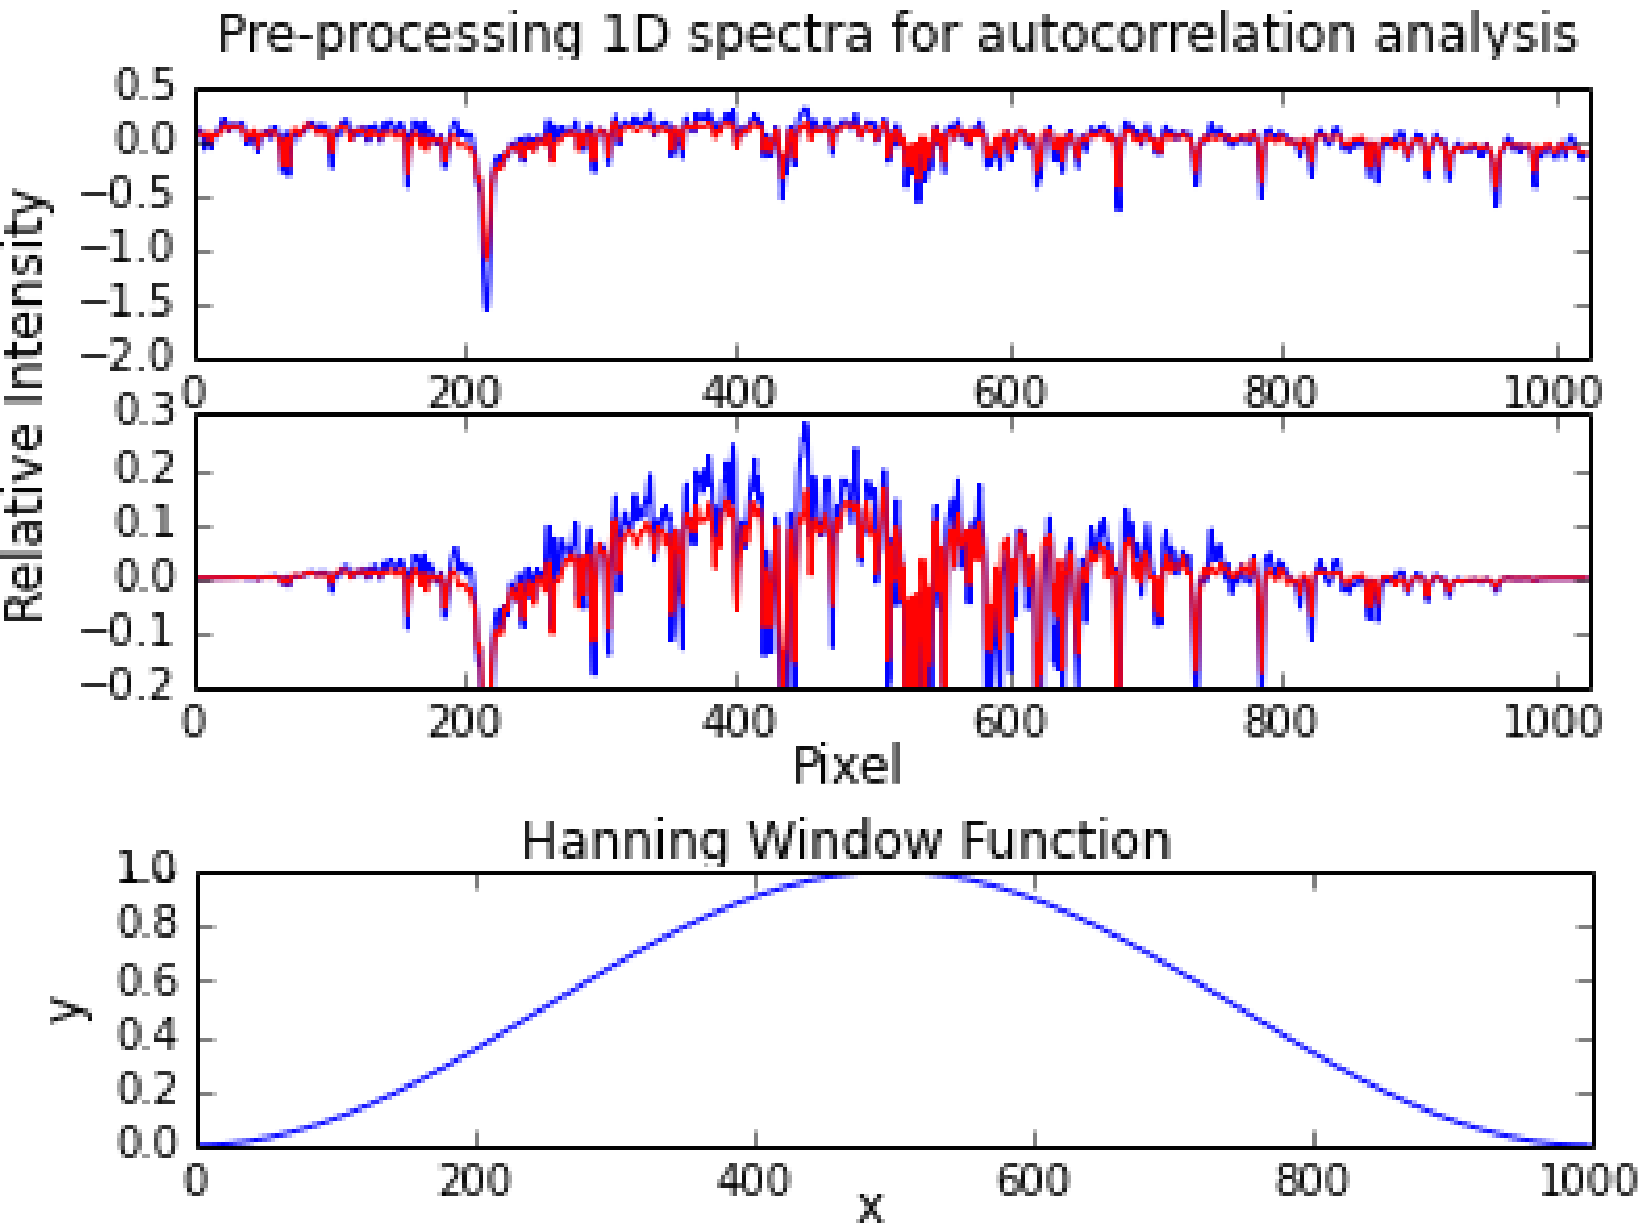
\includegraphics[width=0.5\textwidth]{figures/process_corr_spectra}
\caption{Preprocessing procedures: Mean subtraction and window weighing of spectra.}
\label{process_corr_spectra}
\end{figure}

We find that the centroid value computed is highly sensitive to the choice of region over which the centroid is computed. Given that we are trying to measure the fractional pixel width, there is no point of using a larger range containing assymetrical values about the zero pixel lag that will affect our computed centroid value. Since the spectras are stored in arrays , which can only be shifted an integer number of pixels, any choice of centroid computing region below 1 pixel \\would yield an undesirable result. Therefore, for most of the centroid computed for this lab we used a range of -2 to 2 pixels as shown in right panel in Fig.\ref{autocorr_curve}. 
\begin{figure}[h!]
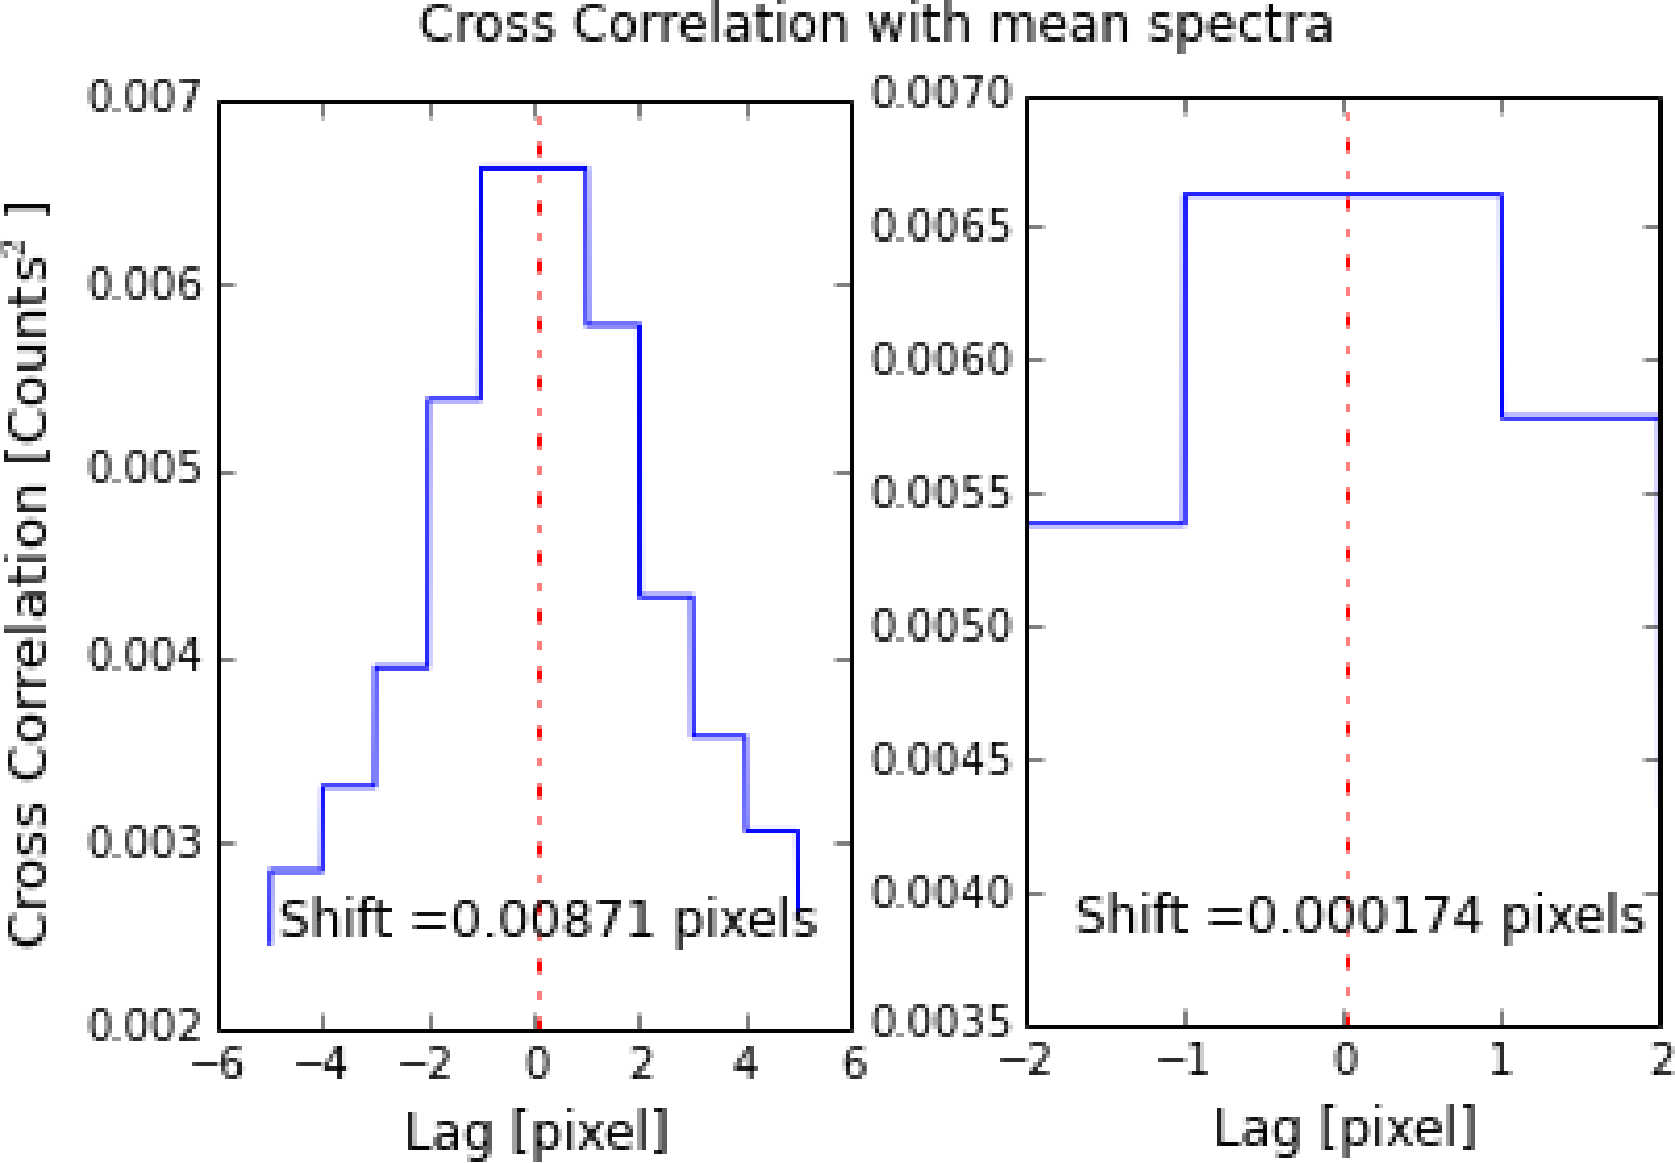
\includegraphics[width=0.5\textwidth]{figures/autocorr_curve}
\caption{ The left figure demonstrates that there is a maximum pixel lag where the shifted and mean spectra that are best correlated. The right figure shows the range used to compute most centroids in this lab.}
\label{autocorr_curve}
\end{figure}
\section{Results}
\subsection{Doppler velocity calculation}
\label{results}
\begin{figure}[h!]
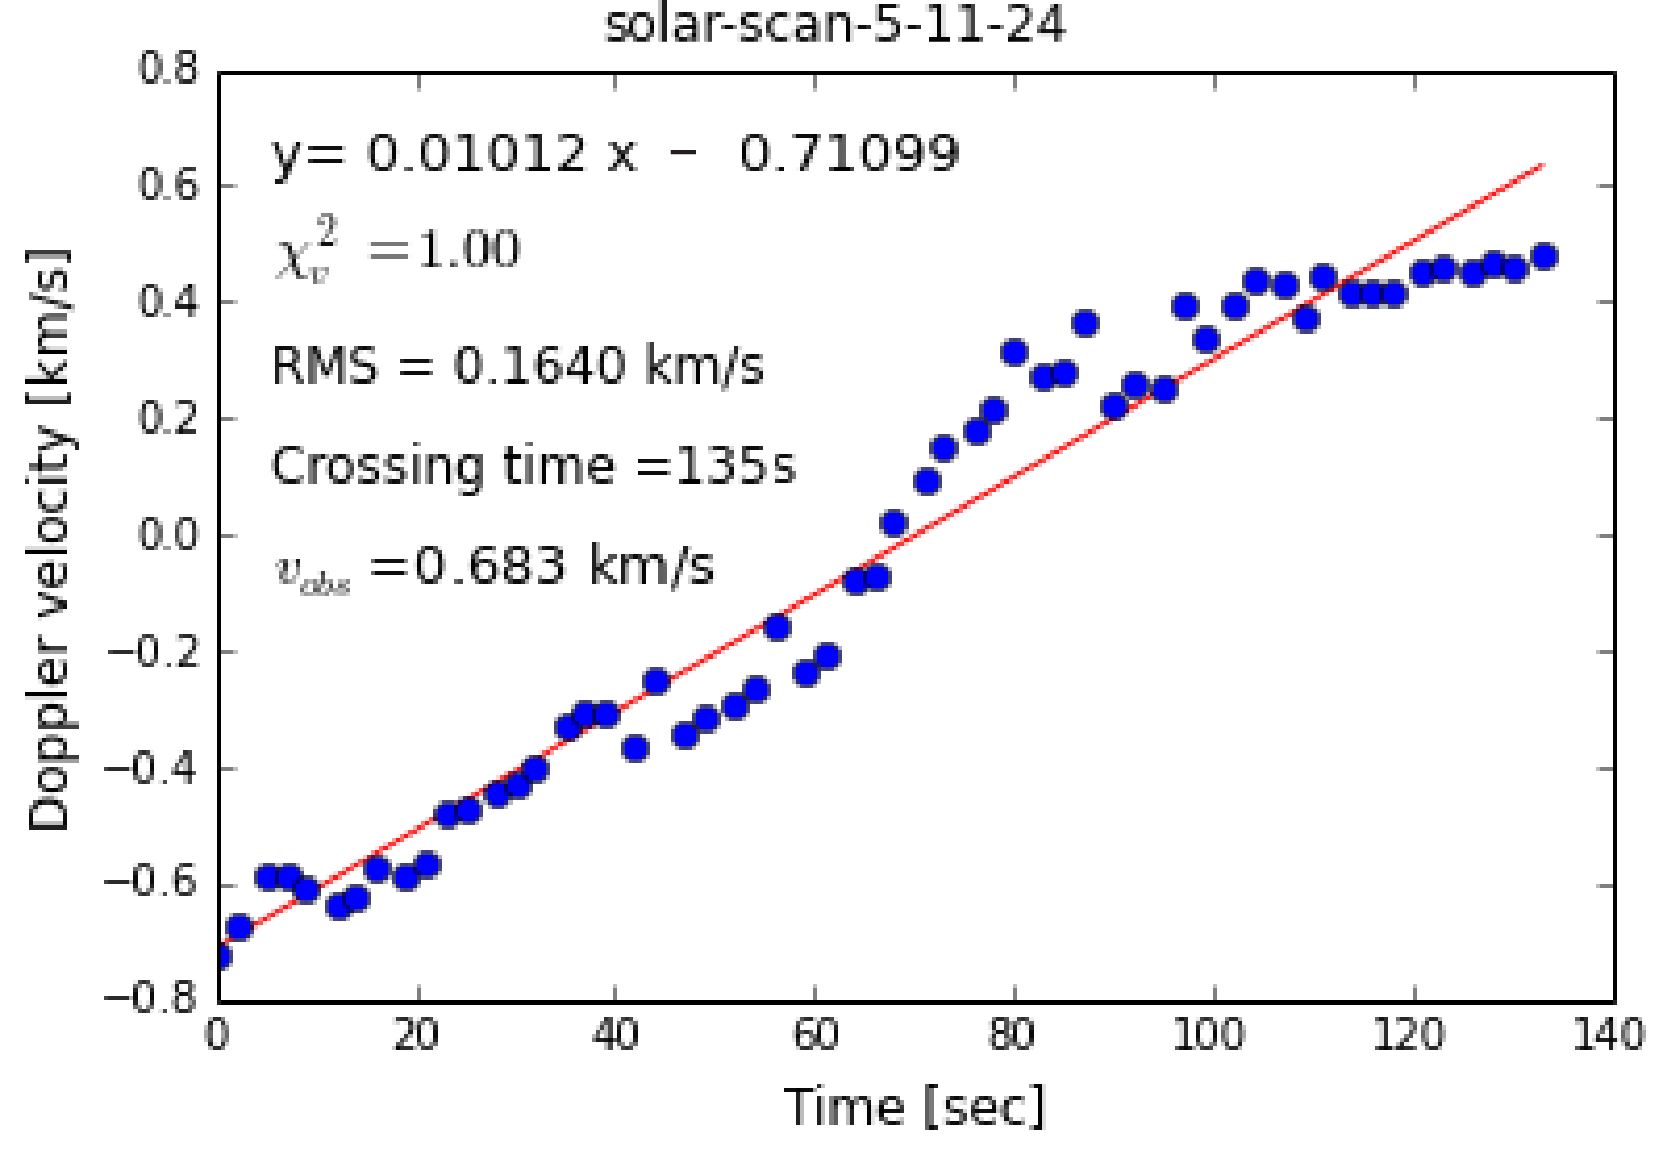
\includegraphics[width=0.5\textwidth]{figures/long_cord_dv}
\caption{Velocity-time graph for a single solar scan with the slope found by linear regression.}
\label{long_cord_dv}
\end{figure}
\begin{figure}[h!]
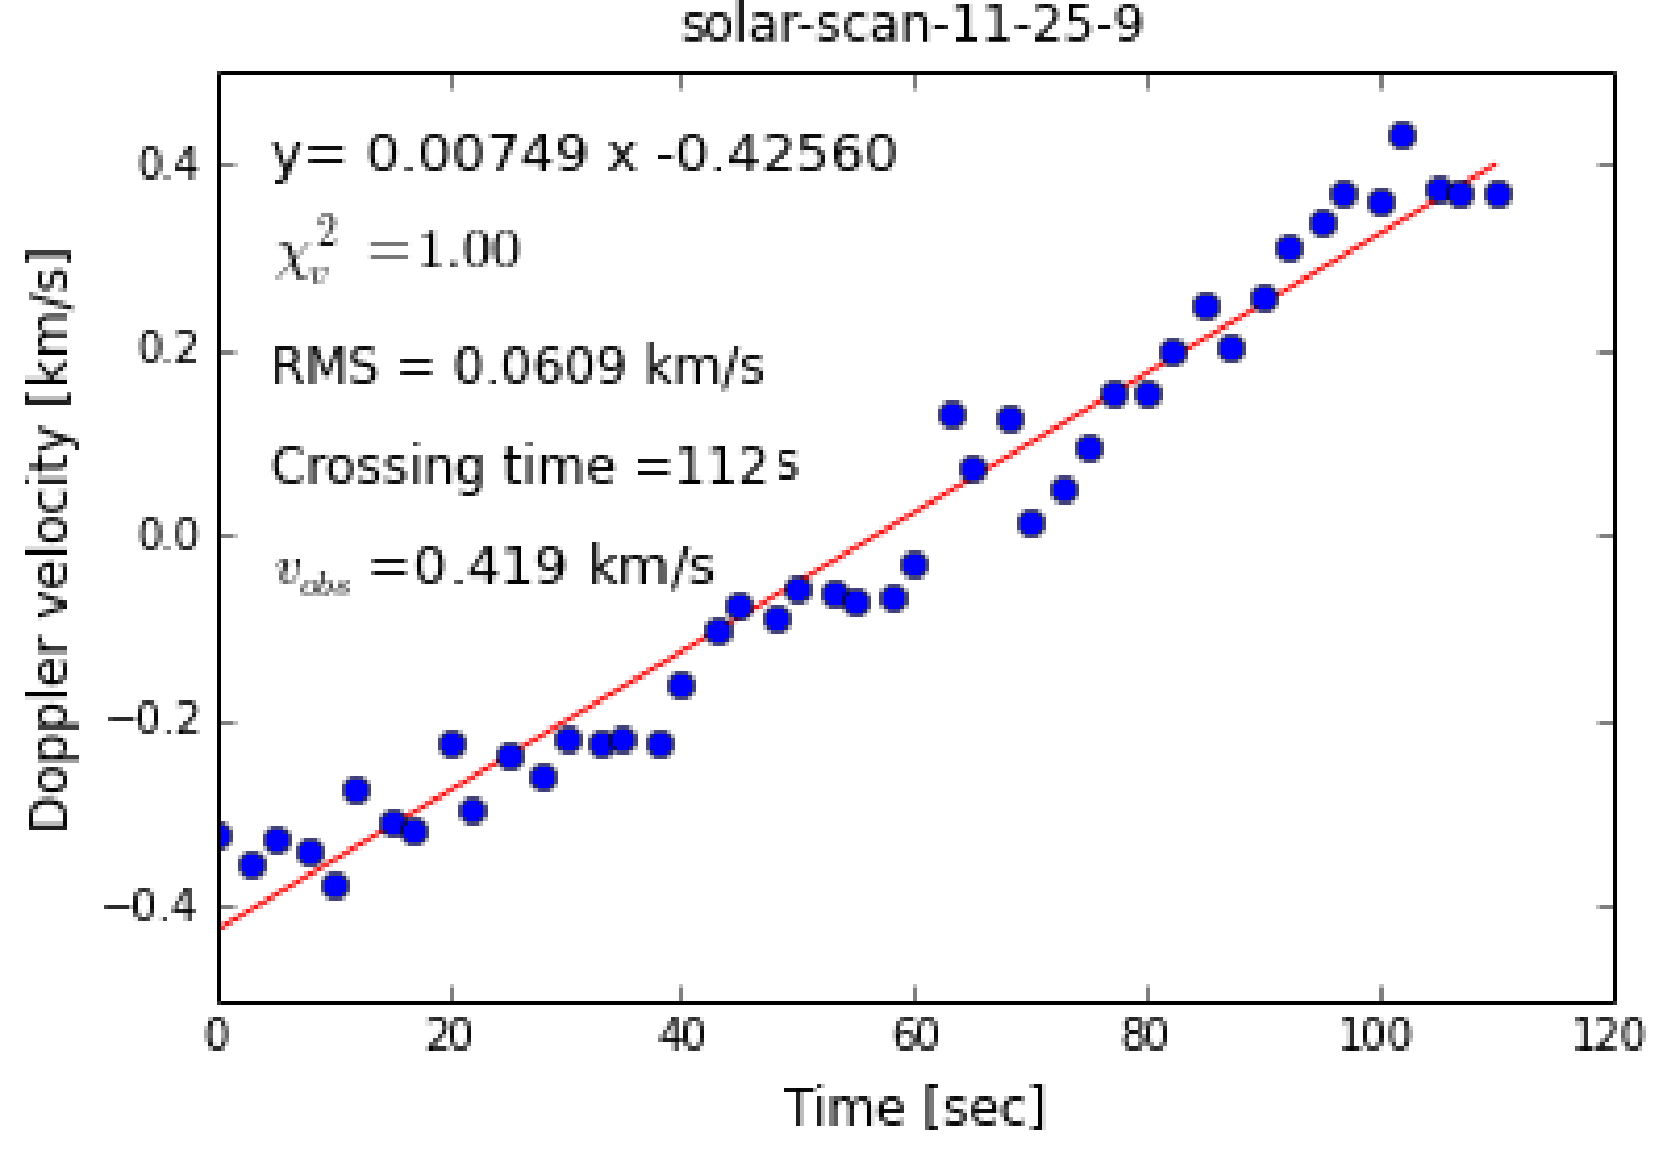
\includegraphics[width=0.5\textwidth]{figures/short_cord_dv}
\caption{The result from a scan with a shorter crossing time than in Fig.\ref{long_cord_dv}, which means that the chord traversed on the Sun's disk is shorter. Different regions of the Sun actually rotates at different rates at different latitudes due to thermal convection, but if we ignore that effect, we should get a smaller radial velocity for our shorter chord scans. The effective radius at that location is closer to the solar spin axis, therefore assuming $\omega$ is constant $v=R\omega$ informs us that we should get a smaller velocity.}
\label{short_cord_dv}
\end{figure}
\label{results}
For each exposure in the cross-correlation analysis, we obtain a pixel value shift ($\Delta x$)that we can convert to the Doppler velocity (v) by (derived from lab handout): 

\begin{equation}
v = c\frac{\Delta\lambda}{\lambda}=c \frac{\frac{d\lambda}{d(\text{pixel})}\Delta x}{\lambda}
\label{doppler_eq}
\end{equation}
%\delta\lambda=\frac{v}{c}\lambda_0
where $\frac{d\lambda}{d\text{pixel}}$ is the dispersion given by Eq.\ref{calib_eq} yielding the corresponding wavelength shift ($\Delta \lambda$), $\lambda$ is the wavelength for the spectral lines, and c is the speed of light.


Excluding the saturated or partially shaded \footnote{The shading effect could be seen from the decrease in intensity in the middle of the scan in the time series plot, which is clearly not an effect of limb darkening.} solar scans, we conducted this analysis on 8 datasets of the same order. Since the crossing time of the scan depends impact parameter of the observer's line of sight, different scans should have the approximately gradient despite the different chord lengths from  each drift scan. The standard deviation of the all the gradients obtained \footnote{with one outlier removed} is 0.0015 km/$s^2$, which shows that the gradients are fairly constant, with an average value of 0.0118 km/$s^2$. 

These gradients are used to calculate the observed velocity at the limb of the Sun by multiplying with the half crossing time (i.e. time for drift scan to drift from center to limb)
This procedure, combined with the model fit for crossing time determination, is more statistically robust than simply taking the first and last Doppler velocities of the solar scan, since it is a continuous approximation of the velocity rather than a discrete selection . Also, due to the limbing effect, there are less photons received on the edges. Therefore, the errors on the velocity values measured are larger, which makes the single measurements even more unreliable to use.
\subsection{Coordinate transformation}
The purpose of solar coordinate transformation is to convert the our $v_{\text{observed}}$ obtained from Doppler shift measurements to the actual radial velocity corrected for our viewing angle.
We make use of the rotational matrix (Eq.\ref{rotmatrix1}) from the lab handout to transform our $v_{\text{observed}}$ to adjust for the fact that the Sun's rotational axes is not perpendicular to the ecliptic (i.e. the observer on Earth is not looking straight on the Sun's equator resulting in a nonzero impact parameter).
\begin{equation}
\bBigg@{4}(\begin{matrix}
\cos\xi & 0 &\sin\xi \\ 
0 &1  &0 \\ 
-\sin\xi &0  &\cos\xi 
\end{matrix}\bBigg@{4})
\label{rotmatrix1}
\end{equation}
where  $\xi$ is the  observer sub-latitudes
Next, we reorient the spin axes of the Sun so that it points N/S by the second transformation matrix: 
\begin{equation}
\bBigg@{4}(\begin{matrix}
1& 0 &0 \\ 
0 &\cos\eta  &\sin\eta \\ 
0 &\sin \eta  &\cos\eta 
\end{matrix}\bBigg@{4})
\label{rotmatrix2}
\end{equation}
where $\eta$ is the North pole angle describes tilt of the Sun's axis of rotation
We obtain the  $\eta$  and $\xi$ from the JPL Horizon web interface.



By conducting these coordinate transformation on the mean observed velocity calculated in Sec.\ref{results}, we obtain 1.257\rpm 0.0185 km/s for the solar radial velocity. The radius of the Sun ($R_{\odot}$) can be obtained by Eq.\ref{sun_size} derived from the lab handout.
\begin{equation}
R_{\odot} = \frac{T_{rot \odot} V_\odot}{2\pi}
\label{sun_size}
\end{equation}
where $T_{rot \odot}$ is the rotational period of the Sun ($\approx$25 days) and $V_\odot$ is the radial velocity at the limb of the Sun. Using the radial velocity from our Doppler measurements, the value radius value of 453855 \rpm 6675 km. Possible deviations from the nominal value ($R_\odot$= 695800 km) are explained in the next section.
\label{size_calc}
\subsection{Error Propagation}
The RMS residual computed for each scan (as quoted in Fig.\ref{long_cord_dv} and \ref{short_cord_dv}) informs us on how much the data  deviates from the model and yields an estimate of how good the linear fit is.  Using the least squares method on the linear model y=a+bx, we can derive an analytical relation to obtain the slope b as well as the error on the value of the slope as described by Press and Vetterling\footnote{Eq.\ref{ls} is an expanded form of  Eq.15.2.9 in the referenced text.}  (1992): 
\begin{equation}
\sigma_b^2 = \frac{\sum\limits_{i=1}^N\frac{1}{\sigma_i^2}}{\sum\limits_{i=1}^N\frac{x_i^2}{\sigma_i^2}\sum\limits_{i=1}^N\frac{1}{\sigma_i^2}-\Big(\sum\limits_{i=1}^N\frac{x_i}{\sigma_i^2}\Big)^2}
\label{ls}
\end{equation}
This value is computed by the a part of the regression algorithm\footnote{\texttt{scipy.stats.linregress}}, the average error on the slope is 0.000276km/$s^2$. The error is propagated when deriving the limb velocity to obtain the value of observed velocity  0.3799 \rpm 0.0185 km/s. Similarly using Eq.\ref{doppler_eq}, we obtain an estimate of the error on the solar radius as 6675.279km.
\section{Conclusion}
In this experiment, we captured the CCD images resulting from a spectrograph while the Sun drifts across the fiber aperture. We perform the routine procedures of background subtraction using darks, bias and flat frames and wavelength calibration using method of linear least squares. We compute the total intensity incident on the spectrometer during the full solar crossing and observed the phenomenon of limb darkening. By using the intensity description given by the Eddington approximation for a grey, plane parallel stellar atmosphere, we obtain the crossing time for the sun to drift across the fiber aperture. 

Converting the 2D CCD image intensity values into 1D spectra, we can conduct the method of cross correlation on multiple data sets. First, we pre-process the spectra by mean subtraction and weighing by window function to assist with finding a fractional pixel shift. Then, by shifting the 1D spectrum by different pixel lags, we can obtain the pixel lag that yields the best correlation results with the mean spectra.

We can deduce the velocity at the limb by multiplying the half crossing time by the slope of a velocity-time graph plotted for the whole scan, which is constant for any set of observation. We can then convert this pixel shift to a observed velocity  at the solar limb using the pixel per wavelength factor acquired  from wavelength calibration and the Doppler velocity formula. Finally, we transform this observed velocity to the solar radial velocity to adjust for the non-zero viewing angle and the tilt of the solar spin axis. This analysis is \\conducted on 8 different solar scans on November 24 and 25, 2014 on the same order and we obtain a solar radial velocity of 1.257 \rpm 0.0185 km/s  which translates to a solar radius of 453855 \rpm 6675 km.

Even the upper estimate of the measured quantities yields a 33.8\% error on the final computed value for the solar radius. One possible sources of error in our analysis is the choice of  $\lambda$ quoted in Eq.\ref{doppler_eq}. Since we have conveniently used m=35, we simply set $\lambda$the 632.8nm of the laser. The choice of $\lambda$ within the range of \rpm 10nm (a single echelle order spans 20nm) does not significantly change ($\approx$\rpm 0.005 km/s). As an extension to the work on this lab, precision can be improved if we cross correlate single spectral lines rather than the whole 1D spectra. In that case, a more accurate value of $\lambda$ can be obtained.

  Another precision improvement step that can be an extension of this lab is to calibrate the wavelength on other orders to increase the number of spectral lines used for each cross correlation analysis. In this lab, we conveniently chose to use the 35$^\text{th}$ for conducting the doppler velocity determination. By doing this on other orders, we can increase the number of spectra used for the correlation analysis for the given data sets that we acquired, thereby increasing the S/N ratio and decreasing the quoted error bar on the measurement.  

 \section*{References}
 \begin{footnotesize}
 \begin{itemize}
 \item Carroll, Bradley W., and Dale A. Ostlie. \textit{An Introduction to Modern Astrophysics}. San Francisco: Pearson Addison-Wesley, 2007. Print.
\item Chromey, Frederick R. \textit{To Measure the Sky: An Introduction to Observational Astronomy}. Cambridge: Cambridge UP, 2010. Print.
\item Press, William H., and William T. Vetterling. \textit{Numerical Recipes in C: The Art of Scientific Computing}. Cambridge University Press, 1992.  
\end{itemize}
% \bibliography{references}
%\bibliographystyle{elsarticle-harv}
  \end{footnotesize}

\end{document}
